\subsection{Results}

The goal has not been reached. However we have been able to see whether a button is pushed or not.\\
Obviously our project works when a consumer infrared is used, such as remote control for a tv, or a dvd player.\\
We found our system doesn't works on home gate remote controls or car keys because those kind of remote controls use signals out of the infrared trasmission(such as Megaherz transmission).\\
Following images show our sampling on different buttons of the remote control Samsung AK59-00149A.\\ 

\begin{figure}[h]
	\centering
	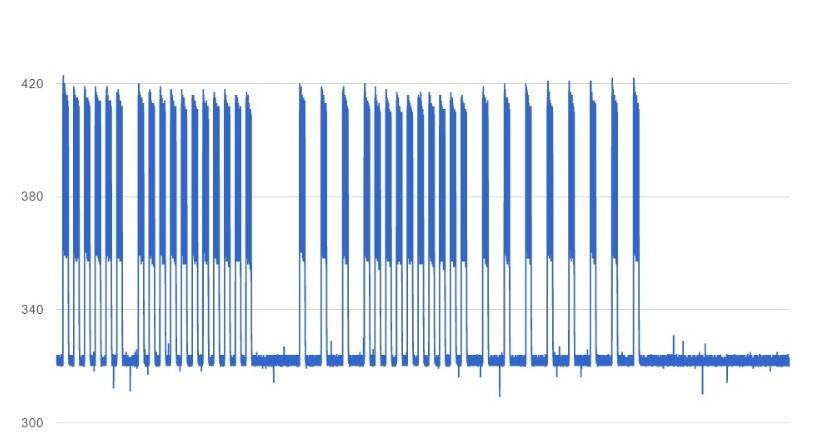
\includegraphics[scale=0.5]{graphs/onButton_2.jpg}%
	\caption{button "ON/OFF"}

\end{figure}

\begin{figure}[h]
	\centering
	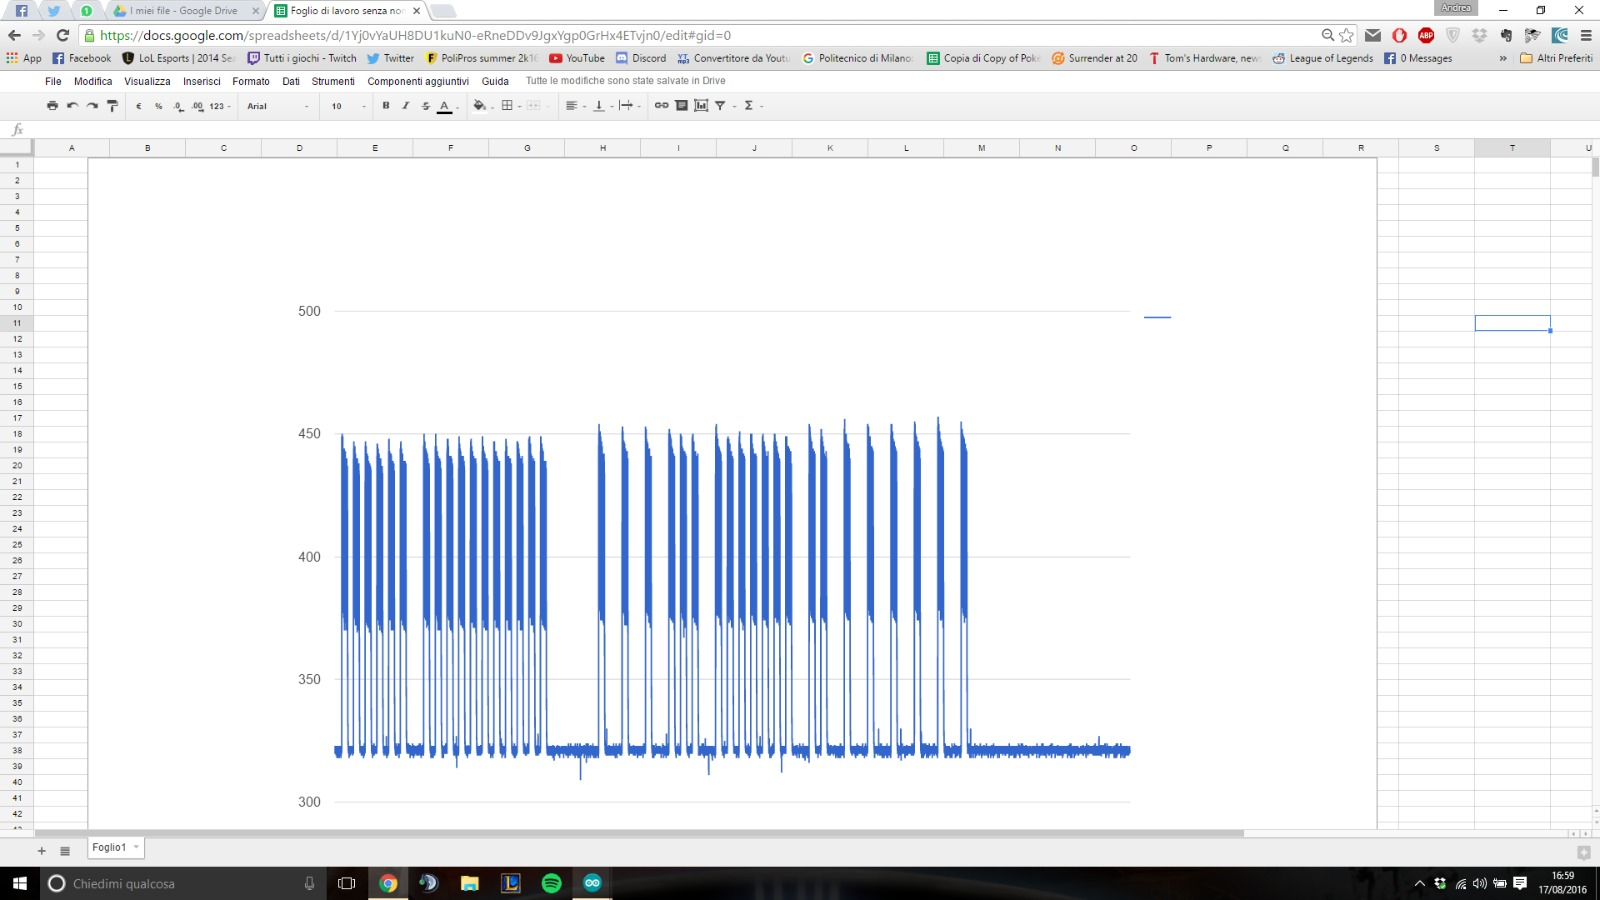
\includegraphics[scale=0.5]{graphs/1Button.jpg}%
	\caption{button "Channel 1"}
		
\end{figure}

\begin{figure}
	\centering
	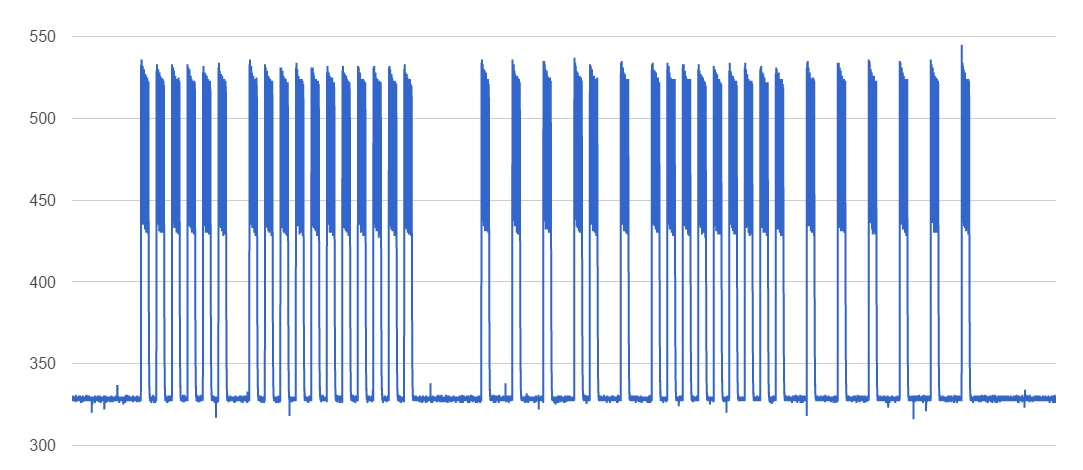
\includegraphics[scale=0.5]{graphs/button2.jpg}%
	\caption{button "Channel 2"}
	
\end{figure}
 How we can see there exist a part at the beginning of the code, the header, that is equal for every button of the same remote control, but the central part is different to recognize several button.